\documentclass[11pt]{article}
\usepackage[utf8]{inputenc}
\usepackage[numbers, square]{natbib} % authoryear, numbers, round, square
\usepackage{amsmath,amssymb}
\usepackage{geometry}
\usepackage[colorlinks=true, allcolors=blue]{hyperref}
\usepackage{bm}
\usepackage{enumitem}
\usepackage{graphicx}
\usepackage{tabularx}
% \usepackage{float}
\geometry{margin=1in}

\usepackage{booktabs}
\usepackage{multirow}
\usepackage{tcolorbox}

\usepackage{lineno}
\linenumbers

\title{%
Enhancing Fluvial Flood Inundation Mapping Through Stochastic Rating Curve Representation
}

% \author{
%   Mohammad H. Erfani\thanks{\texttt{moerfani@ucsd.edu}} \\[0.3em]
%   \small Center for Western Weather and Water Extremes (CW3E) \\
%   \small Scripps Institution of Oceanography \\
%   \small UC San Diego
% }
% \date{}

\begin{document}
\maketitle

\begin{abstract}
In river systems, the stage--discharge relationship plays a crucial role in flow characterization and streamflow estimation. Conventionally, this relationship is estimated using rating curves expressed as a fixed functional form. This deterministic approach may not adequately explain or account for the inherent uncertainties in the stage-discharge relationship, which may arise from changes in hydraulic characteristics, morphological alterations in the riverbed, and anthropogenic modifications. This study proposes a stochastic approach that can effectively account for the uncertainties associated with the stage--discharge relationships. For this purpose, a copula-based Bayesian framework selects the best-fitting copula family from several candidates to characterize the joint stage–discharge dependence. An analysis of 6,323 USGS gauges across the contiguous United States shows that this stochastic behavior is widespread, not confined to a few sites. Results demonstrate that the copula-based framework can effectively capture the range of stage--discharge variations, which deterministic approaches fail to represent. Applied across sites of varying drainage area, stream order, and hydrologic setting under a single uniform configuration, the framework produced well-calibrated predictive intervals, with 95\% coverage between 94.1\% and 97.8\%. We also demonstrate the practical implications of this approach by integrating the resulting probabilistic rating curves with a conceptual flood inundation model to show how stage uncertainty can impact the inundation extents. These findings show that accounting for uncertainty in natural systems yields a more realistic, interpretable representation, particularly for stage–discharge relationships where probabilistic modeling captures the drivers of stochastic behavior.
\end{abstract}

\section{Introduction}
Rivers are essential components of hydrologic systems, transporting water through the channels and floodplains. They are naturally dynamic, as they evolve in response to changes in channel morphology, fluctuations in discharge, and sediment transport \cite{rhoads2020}. These changes alter a river's hydraulic behavior, so the same discharge does not always correspond to the same water level. Understanding the stochastic behavior of rivers can significantly improve flood mitigation, infrastructure design, water-supply planning, and ecological stability \cite{arnell2016}.

A common simplification to understand flows in rivers involves the use of rating curves to represent the stage--discharge relationship. The rating curve relates stage (water level) to streamflow (discharge) and is typically expressed as a deterministic function, unique to each gauging station for a given period of time. However, this formulation carries several limitations, as it fails to capture the inherent complexities of sediment transport and hydraulic characteristics. More critically, the stage--discharge relationship is stochastic in nature, and deterministic formulations cannot account for the drivers of this stochasticity. These drivers include, but are not limited to, hysteresis effects during unsteady flow events, particularly those driven by intense precipitation or reservoir releases~\cite{perret2022, fread1975}; complex boundary conditions such as backwater effects~\cite{hidayat2011} and seasonal vegetation growth~\cite{perret2021}; and anthropogenic modifications. Consequently, deterministic rating curves fail to represent the inherent uncertainties that are critical for accurate discharge estimation in river systems.

Several studies have improved the representation of stage--discharge relationships. These include recalibrating curve coefficients, adjusting roughness values, and using limited cross-sectional or remotely sensed data to better represent channel geometry~\cite{Singh2010, Barbetta2012, Pan2016}. The deterministic approach was further enhanced by incorporating higher-order formulations, such as polynomial, spline-based, or hydraulically informed models, as well as data-driven and machine learning approaches that estimate rating curve parameters from geomorphic and hydrologic attributes at local to continental scales~\cite{Fenton2018, Lee2021, Pati2023, chang2023, Baruah2025}. Despite improving local accuracy in specific settings, these methods result in a unique stage for every discharge, which may not reflect the inherent uncertainty in the stage-discharge relationship. This limitation becomes challenging, particularly at high flows, where direct measurements are scarce, and the curve may have to be extrapolated beyond the observed range~\cite{petersen2009}. A probabilistic framework that can characterize the uncertainty of the stage-discharge relationship offers more reliable discharge estimations.

To overcome these limitations, likelihood-based and Bayesian frameworks have been developed to explicitly quantify stage–discharge uncertainty by modeling measurement error, hydraulic variability, and complex channel controls~\cite{lecoz2014, mansanarez2016, mansanarez2019, ocio2017}. These approaches include joint likelihood formulations that simultaneously estimate rating-curve and flood-frequency parameters~\cite{petersen2009}, Bayesian inference schemes that incorporate hydraulic priors and gauging uncertainty~\cite{lecoz2014}, and methods that address backwater effects, unstable channels, and epistemic uncertainty~\cite{mansanarez2016, mansanarez2019, westerberg2015, reitan2008}. Collectively, these methods quantify discharge uncertainty and demonstrate that rating-curve uncertainty propagates substantially into downstream hydraulic estimates~\cite{petersen2009, ocio2017}.

Despite these advances, existing probabilistic methods still assume a prescribed functional form for the stage--discharge relationship, typically a single- or multi-segment power law. Uncertainty is then represented around this prescribed function, either through the distribution of its parameters or through additional error terms~\cite{lecoz2014, reitan2008, mansanarez2016, mansanarez2019, mcmillan2015}. Many of these methods require site-specific hydraulic priors and expert knowledge of channel controls to constrain their estimates, which limits their scalability across diverse settings and large river networks~\cite{lecoz2014, mansanarez2019}. Less attention has been given to frameworks that treat discharge and stage as jointly distributed random variables. Such an approach would characterize their dependence structure directly from observations.

This study introduces a copula-based probabilistic framework for characterizing the stage--discharge relationship in natural river systems. Drawing from multivariate probability theory and Bayesian networks, this approach models discharge and stage as jointly distributed random variables and estimates the conditional distribution of stage given discharge, $f(H|Q)$, directly from field observations. The IFMHA dataset, which provides extensive event-level hydraulic measurements across diverse channel types, serves as the observational basis for fitting and evaluating the proposed framework~\cite{Erfani2024}. To investigate the practical implications of this approach, the resulting probabilistic stage estimates are integrated with the Office of Water Prediction (OWP) Height Above Nearest Drainage (HAND) Flood Inundation Mapping (OWP HAND-FIM) model, demonstrating how uncertainty in the stage--discharge relationship propagates into spatially distributed inundation extents. The framework captures the natural variability of the stage--discharge relationship directly from observations, and as it requires no prescribed functional form or site-specific hydraulic knowledge, it can be applied across diverse channel types and large river networks.

\section{Dataset Description} \label{sec:dataset}
This study uses the Inventory of Field Measurements of Hydraulic Attributes (IFMHA) as the observational basis for fitting and evaluating the proposed framework~\cite{Erfani2024}. IFMHA is a national dataset of direct streamflow measurements collected by the U.S. Geological Survey (USGS) at streamgages across the contiguous United States (CONUS). Each record pairs a field-measured discharge with the corresponding observed stage, thereby providing direct information about the stage--discharge relationship. The dataset includes repeated measurements at thousands of streamgages spanning diverse hydrologic, climatic, and channel conditions. Its extensive spatial coverage and large number of site-level observations make it well suited for examining whether variability in the stage--discharge relationship is widespread and for developing a probabilistic representation of that variability.

Here, we first evaluated whether the assumption motivating the framework, that comparable discharges can be associated with different observed stages, is supported by the IFMHA measurements. For each streamgage, discharge observations were divided into within-site deciles, and the interquartile range of stage was calculated within each sufficiently populated decile. The site-level metric was then defined as the mean of the retained decile-level stage IQRs. Thus, larger values indicate greater stage variation among measurements belonging to similar, although not identical, discharge ranges. This diagnostic is used only to characterize streamgage behavior across CONUS. The filtering criteria, mathematical formulation, and limitations of the metric are provided in Appendix~\ref{app:stage_spread_metric}.

Figure~\ref{fig:fig-01} presents the resulting metric for 6,323 USGS streamgages represented in IFMHA. Values near zero indicate that observations at a streamgage closely follow a single-valued stage--discharge relationship, whereas larger values indicate that substantially different stages were observed within similar ranges of discharge. The numerous streamgages with moderate to large values, shown in orange and red, are distributed across multiple regions of CONUS rather than being confined to a small number of isolated locations. This spatially widespread pattern provides empirical evidence that variability in the stage--discharge relationship is a common feature of the observations and is not merely an artifact of a few anomalous streamgages. The results therefore support the central premise of this study: a deterministic rating relationship cannot fully characterize the observed hydraulic behavior at many sites, motivating a probabilistic framework that represents the conditional distribution of stage for a given discharge.

\begin{figure}[hbt]
    \centering
    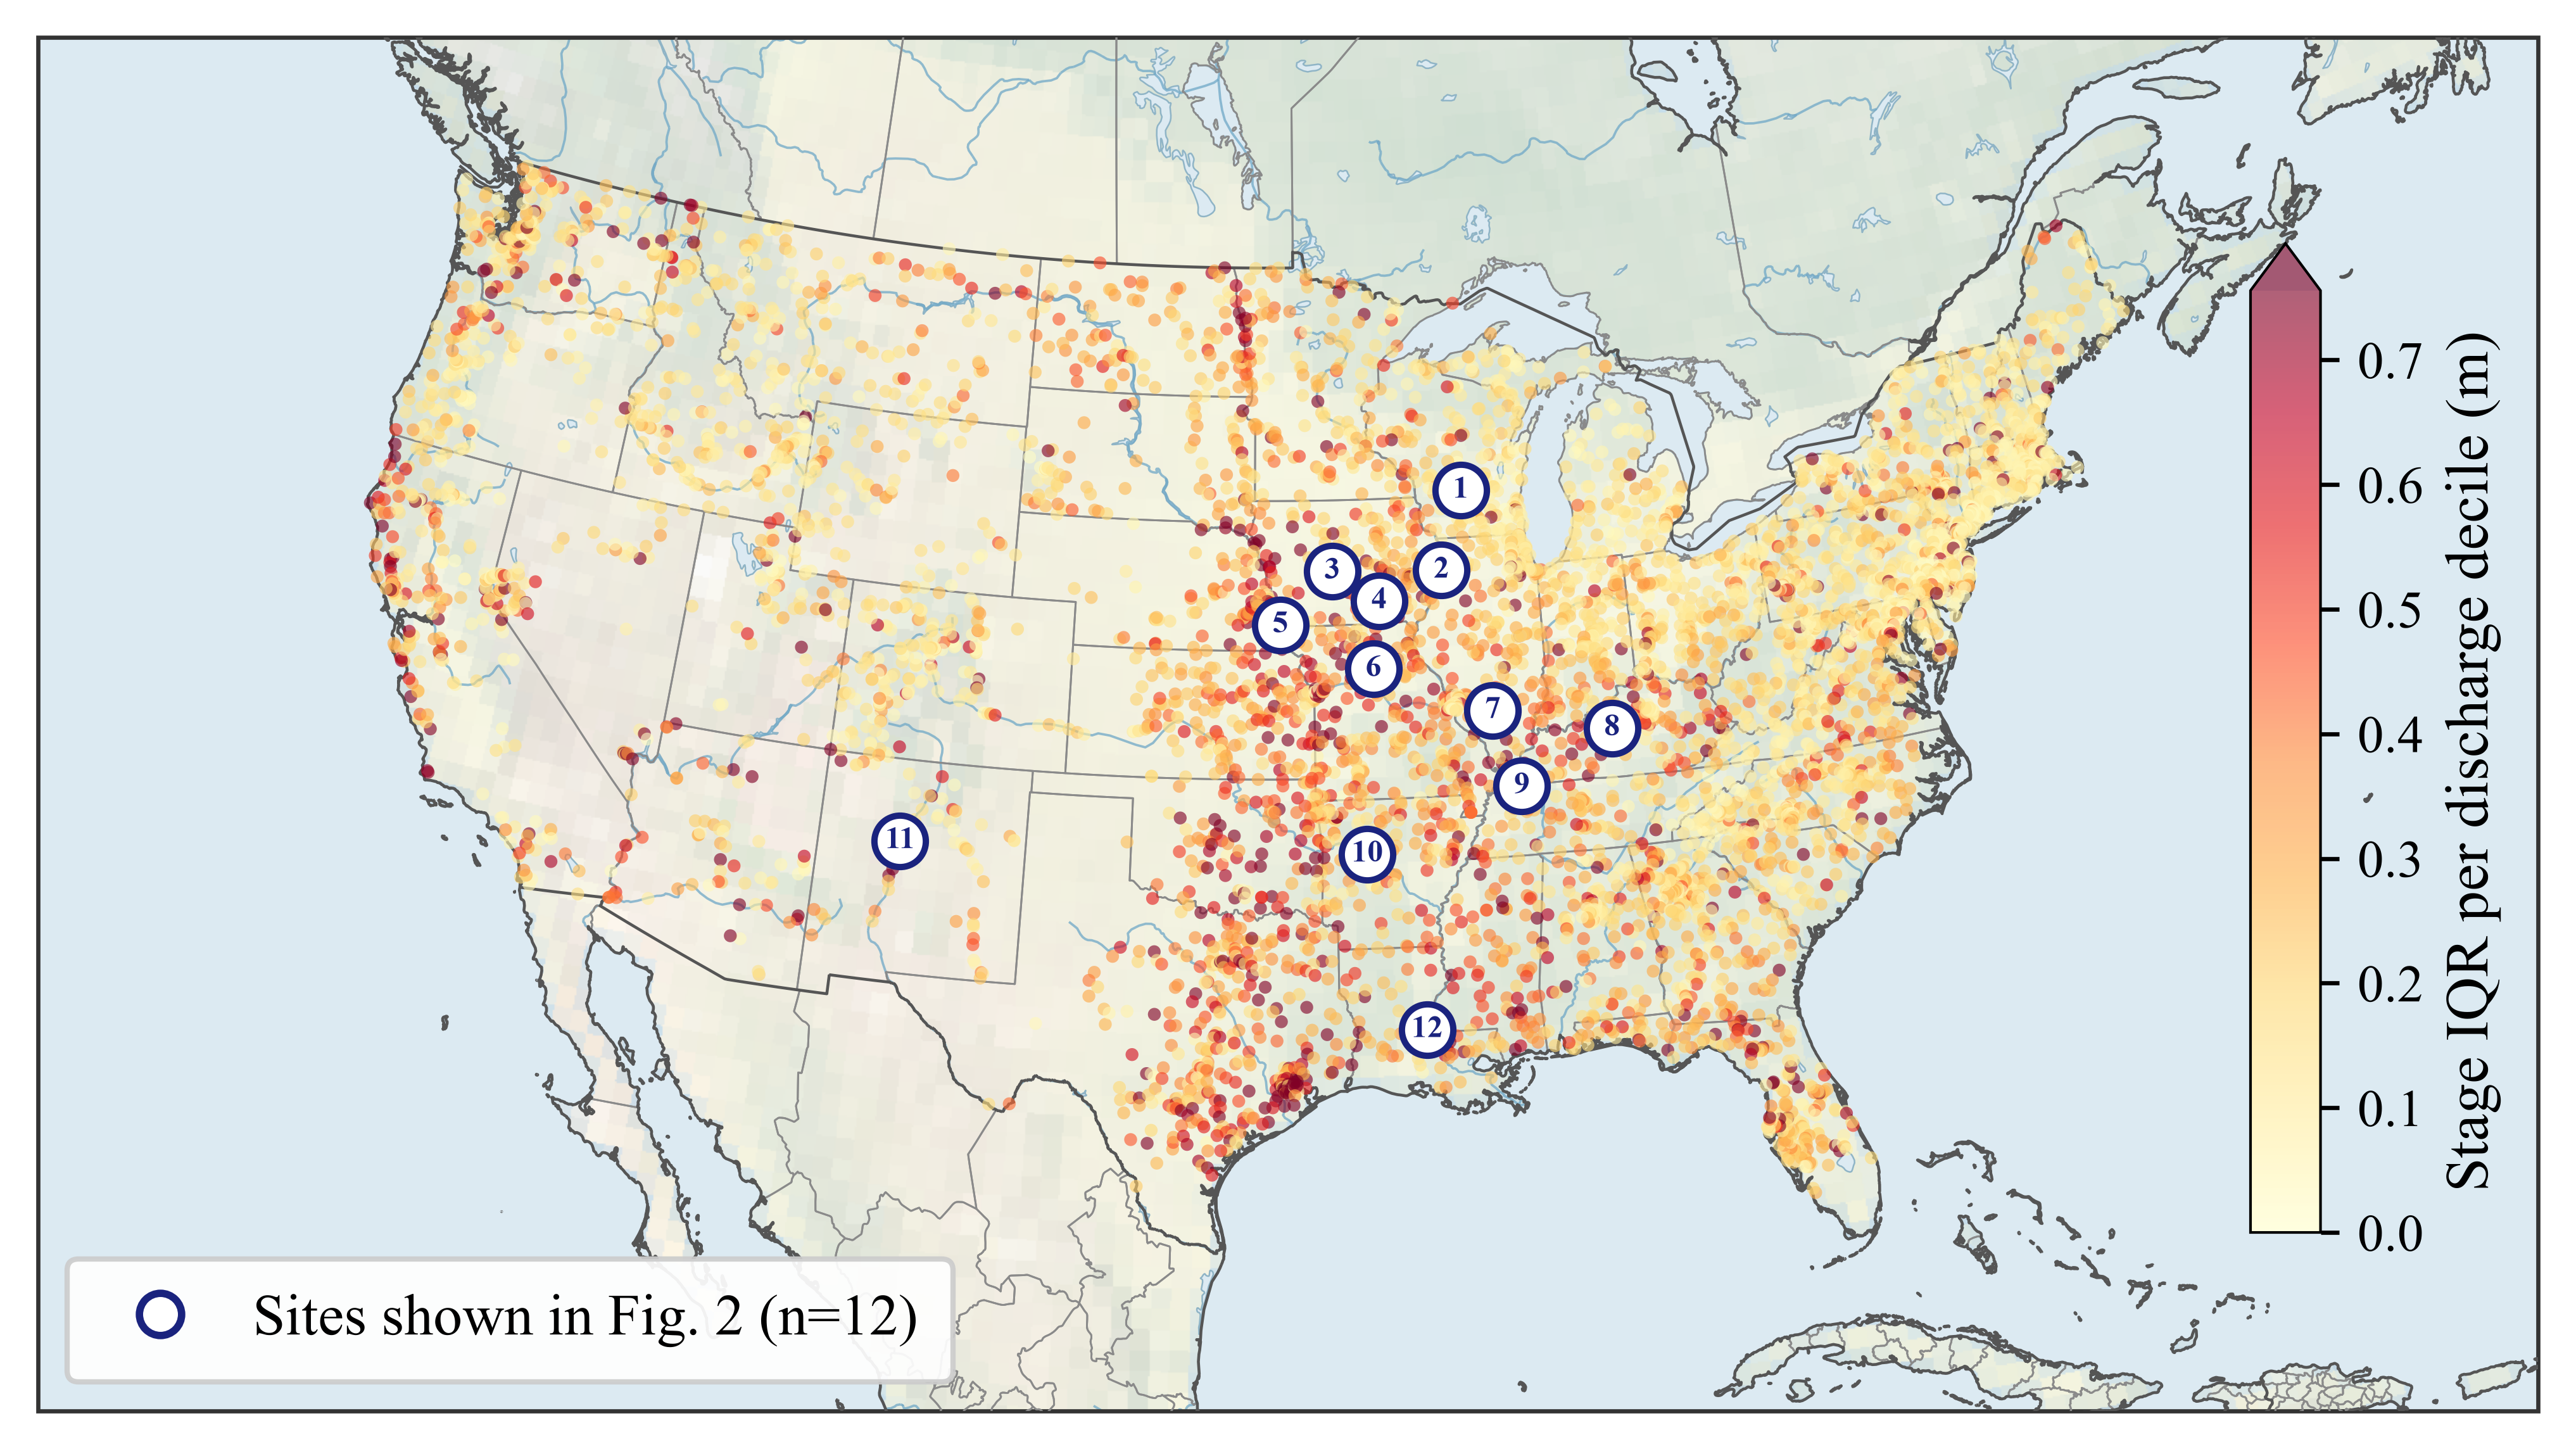
\includegraphics[width=\textwidth]{figs/fig-01.png}
    \caption{Site-level stage--discharge variability across 6,323 USGS gauges in the IFMHA dataset.}
    \label{fig:fig-01}
\end{figure}

\section{Methodology}
This section describes the three main components of our analytical framework. We first present a copula-based approach for jointly modeling the stage--discharge relationship. We then describe the OWP HAND-FIM framework, a conceptual ``bathtub'' model used to translate discharge or stage estimates into spatially distributed inundation extents. Finally, we provide a brief overview of Gaussian Process Regression (GPR), which is used as a baseline model to compare the performance of the proposed copula-based framework.

\subsection{Stochastic Characterization of Hydraulic Relationships}
The $Q$--$H$ relationship is stochastic in nature, and the modeling framework therefore utilizes a probabilistic representation to remain physically consistent~\cite{Bulygina2011, Bulygina2010}. This relationship is characterized through the conditional distribution $f(H \mid Q)$, derived from the joint bivariate distribution $f(Q, H)$, which captures the nonlinear dependence between discharge and stage directly from observations. 

\begin{equation}
    f(H \mid Q) = \frac{f(Q, H)}{f(Q)}
\end{equation}

\subsection{Copula-Based Joint Modeling}
Copula theory offers a flexible framework for constructing the joint distribution $f(Q,H)$ by separating marginal behavior from dependence structure~\cite{Joe2014}. According to Sklar's Theorem~\cite{Sklar1959}, the joint CDF of discharge and stage can be written as:

\begin{equation}
    F(q,h) = C\!\left(F_Q(q),\,F_H(h)\right)
\end{equation}

where $F_Q$ and $F_H$ are the marginal CDFs of $Q$ and $H$, and $C$ is a copula that captures all dependence between the two variables. The probability integral transform (PIT), defined as $u=F_Q(q)$ and $v=F_H(h)$, maps each variable to the unit interval $[0,1]$ and isolates the dependence structure  from the marginal scales of $Q$ and $H$. The bivariate copula  density is then obtained as~\cite{Sadegh2018}: 

\begin{equation}
    c(u, v) = \frac{\partial^2 C(u, v)}{\partial u \, \partial v}
\end{equation}

The joint density function can accordingly be decomposed as~\cite{Madadgar2013}:

\begin{equation}
    f(q, h) = c(u, v)\, f_Q(q)\, f_H(h)
\end{equation}

where $f_Q$ and $f_H$ are the marginal probability density functions of $Q$ and $H$, corresponding to the CDFs $F_Q$ and $F_H$ defined above. By substituting this expression into the definition of conditional probability, the conditional density of stage given a specific discharge level is derived 
\cite{Madadgar2013, Mazdiyasni2017}:

\begin{equation}
    f(h \mid q) = \frac{c(u, v)\, f_Q(q)\, f_H(h)}{f_Q(q)} = c(u, v)\, f_H(h)
    \label{eq:copula}
\end{equation}

The conditional distribution $f(h \mid q)$ is the key quantity in this framework, providing the full distribution of stage at any given discharge and forming the basis of the probabilistic rating curve. The other components of the framework, including marginal distribution selection, copula selection, and performance evaluation metrics, are described in detail in Appendix~\ref{app:src_development}. It is worth noting that copula-based modeling requires input observations to be independent and identically distributed (i.i.d.) samples from a stationary joint distribution. The $(Q, H)$ pairs used here are field measurements with temporal spacing typically long relative to the hydraulic response time of the channel. They can therefore reasonably be treated as independent. To further reduce short-term autocorrelation, measurements taken on the same calendar day were averaged into a single value, and a minimum three-day gap was maintained between successive observations. This ensures that each $(Q, H)$ pair represents a distinct hydraulic event.


\subsection{Flood Inundation Mapping}
We demonstrate the practical implications of the proposed probabilistic framework by integrating the resulting rating curves with the OWP HAND-FIM framework. The National Oceanic and Atmospheric Administration (NOAA) Office of Water Prediction (OWP) Height Above Nearest Drainage Flood Inundation Mapping model (OWP HAND-FIM) is a rating curve-based flood mapping tool. It provides a well-established platform through which the differences between deterministic and probabilistic stage estimates become directly observable. The HAND approach relates water-surface elevation to inundation extent by using the vertical distance between each terrain cell and the nearest drainage line~\cite{aristizabal2023}.

In the operational HAND--FIM workflow, stage values are typically obtained from a deterministic Synthetic Rating Curve (SRC). SRC applies Manning's equation to terrain-derived channel geometry to map each discharge to a single fixed stage value. We generalize this step by replacing the SRC stage with percentile estimates derived from $f(H \mid Q)$. Mapping each percentile through the HAND--FIM framework yields a corresponding inundation extent. This approach can effectively capture the uncertainty in the stage--discharge relationship. A major advantage of this method is its flexibility: Both the number of maps and the specific percentiles chosen can easily be changed depending on the level of risk to be assessed.

\subsection{Gaussian Process Regression}
Gaussian Process Regression (GPR) is a non-parametric, Bayesian approach to regression that can flexibly model complex relationships between input and output variables~\cite{williams2006gaussian}. In this study, GPR is used as a baseline model to compare the performance of the proposed copula-based framework. GPR assumes that the observed data can be modeled as a realization of a Gaussian process, which is defined by a mean function and a covariance function (kernel). The choice of kernel determines the smoothness and structure of the function being modeled. In this study, we use the radial basis function (RBF) kernel, which is commonly used for its ability to capture smooth variations in the data. The GPR model is trained on the same $(Q, H)$ pairs used for the copula-based framework, and the predictive distribution of stage given discharge is obtained. The performance of GPR is then evaluated using the same metrics as the copula-based framework, allowing for a direct comparison of the two approaches in terms of their ability to capture the uncertainty in the stage--discharge relationship.

\section{Results}
% TODO: add an overview of the results section here

\subsection{Spatial Variability in Rating Curve Behavior}
According to the analysis presented in Section~\ref{sec:dataset}, the stage--discharge relationship exhibits substantial variability across many USGS streamgages in the IFMHA dataset. This variability is examined in relation to the channel and physiographic characteristics based on the fluvial hydraulic and geometry attributes presented in the IFMHA dataset (Table~\ref{tab:tab-01}). To further illustrate this variability, we selected twelve representative sites with different range of variability (numbered in Figure~\ref{fig:fig-01}). Their observed rating curves are shown in Figure~\ref{fig:fig-02}.

\begin{table}[htbp]

    \centering
    \caption{Factors associated with stage--discharge variability.}
    \label{tab:tab-01}
    \begin{tabularx}{\textwidth}{l l X}
        \toprule
        Category & Factor & Relationship to variability \\
        \midrule
        Geomorphic control & Channel material\textsuperscript{a} & Fine, mobile substrate (silt, sand) $\rightarrow$ more variable \\
        & Channel bed stability & Soft, mobile bed $\rightarrow$ more variable \\
        \midrule
        Hydraulic control & Channel slope & Lower gradient $\rightarrow$ more variable \\
        \midrule
        Network-scale control & Drainage area & Larger drainage area $\rightarrow$ more variable \\
        & Stream order & Higher stream order $\rightarrow$ more variable \\
        \midrule
        Data quality & Measurement method & More reliance on indirect methods (cableway, bridge, boat) $\rightarrow$ more variable \\
        \bottomrule
\end{tabularx}

    \vspace{2pt}
    \raggedright\footnotesize\textsuperscript{a}Silt, sand, gravel, cobble, boulder.
\end{table}

\begin{figure}[hbt]
    \centering
    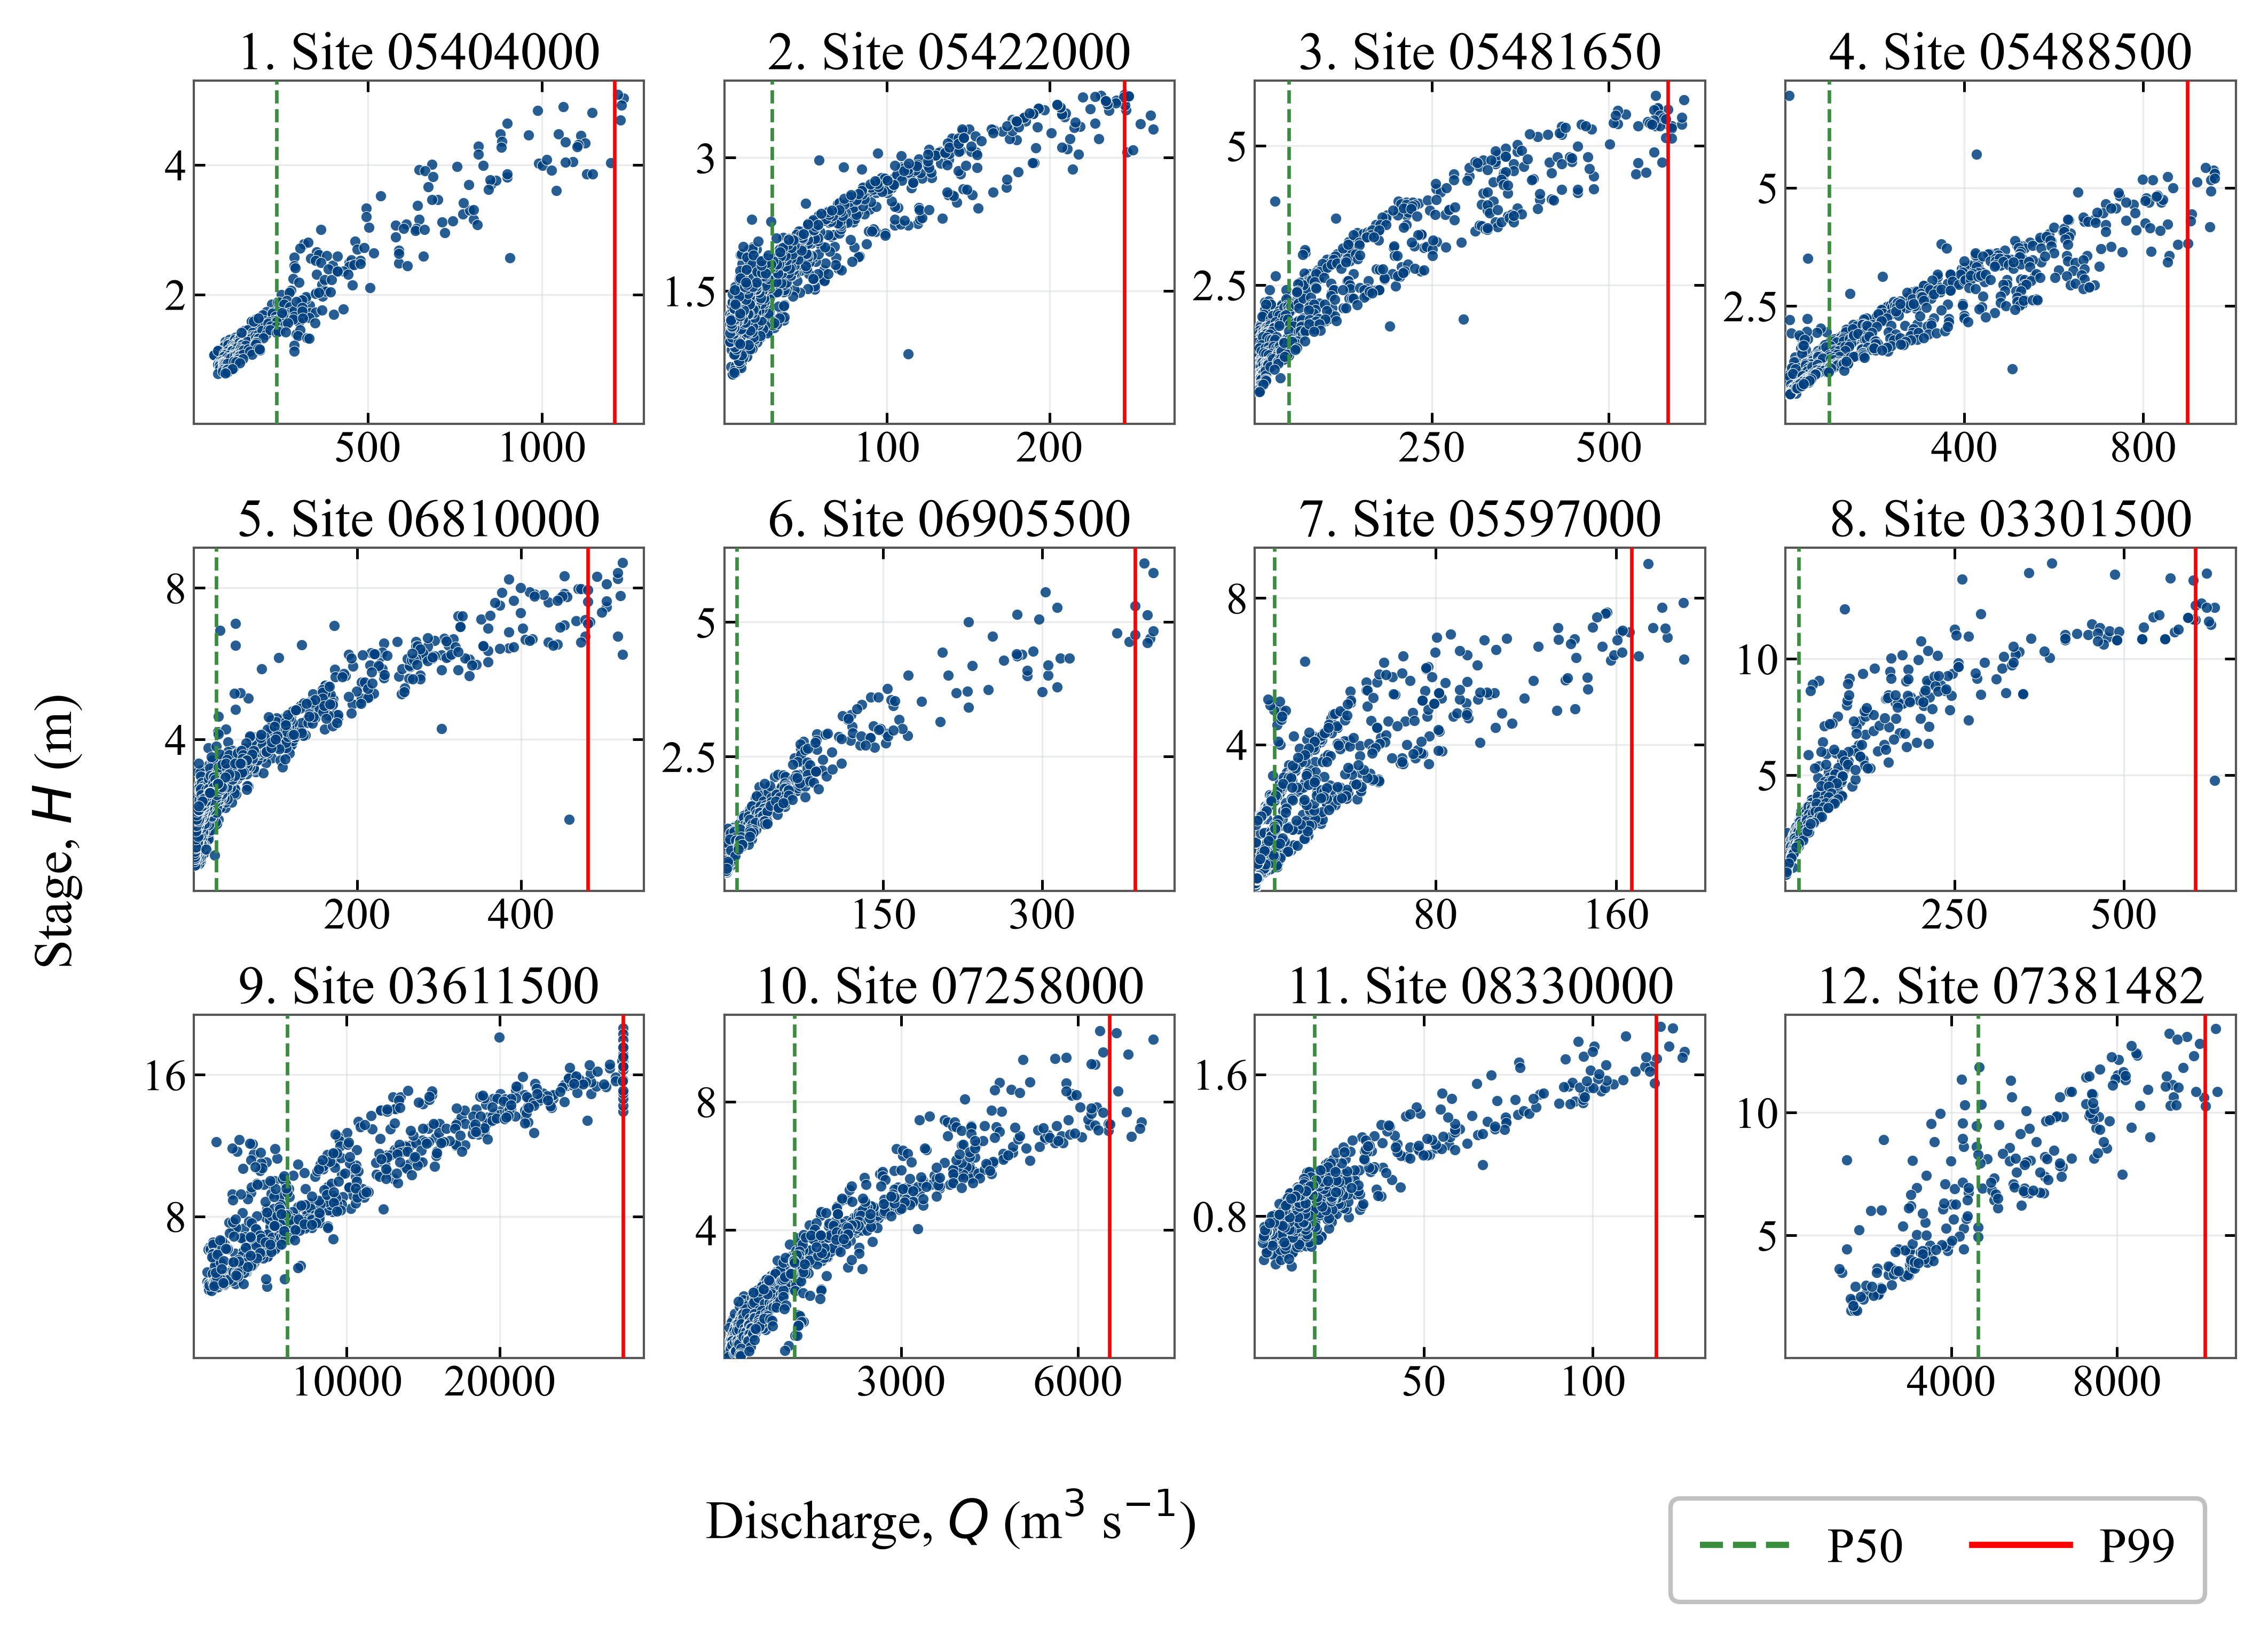
\includegraphics[width=\textwidth]{figs/fig-02.png}
    \caption{Observed stage--discharge rating curves for the 12 sites numbered in Figure~\ref{fig:fig-01}.}
    \label{fig:fig-02}
\end{figure}

Channel material shows the clearest link: gauges on silt or sand substrate have more than double the median variability of gauges on boulder- or bedrock-controlled channels ($0.26-0.31\,m$ versus $0.12-0.14\,m$). Beds of fine, mobile material change shape between measurement visits, as high flows scour sediment away and later flows deposit it again. As a result, the same discharge can produce a different stage on different dates, simply because the bed shape underneath it is no longer the same. Most of the twelve sites examined in this study sit on such beds.

Channel slope shows a similar pattern. Low-gradient channels amplify the sensitivity of stage to discharge. The energy slope enters the governing open-channel flow equations as a square-root term in the denominator. A small change from backwater, an unsteady flood wave, or minor roughness variation can therefore produce a disproportionately large stage response at a given discharge. Larger, higher-order rivers show the same tendency. They are more prone to backwater influence and to hysteresis between the rising and falling limbs of a flood wave. Site 9 drains the largest and highest-order basin among the twelve sites studied here and shows correspondingly high variability; Among the twelve, site 11, with a comparatively steeper reach, shows lower variability.

These factors are not independent. Low-gradient, high-order rivers with large drainage areas tend to also have fine-grained, mobile channel beds. This is why the geographic pattern in Figure~\ref{fig:fig-01} aligns closely with the alluvial lowland regions of the Great Plains and the Mississippi basin. The steep, bedrock- and boulder-controlled channels of the Appalachian and Rocky Mountain provinces show the opposite pattern.

A secondary, non-physical factor likely also contributes. At high flow, measurement crews at these same gauges shift disproportionately from wading to indirect methods such as cableway, bridge, or moving-boat measurement. Site 7 is a clear example where crews rely almost entirely on bridge and cableway measurement once flow rises above its typical range. These methods carry greater uncertainty than direct wading measurement. Part of the high variability at high-discharge, alluvial-river gauges therefore likely reflects the genuine physical processes described above, and part of it likely reflects this added measurement uncertainty. More investigation is provided in Appendix~\ref{app:stage_spread_metric}.

\subsection{Stochastic Rating Curve Representation}
Figure~\ref{fig:fig-03} presents the results of the proposed framework applied to the sites discussed previously. Prior to fitting the framework to each site, we first applied a preprocessing steps which are described in Appendix~\ref{app:preprocessing}. Results are shown as both 50\% and 90\% predictive intervals. Under the more conservative approach (90\% interval), the bands encompass the high-flow observations at nearly all sites. In a few instances such as Site 07258000, where some extreme values fall outside the 90\% band, coverage can be improved by using a higher-coverage predictive interval (e.g., 95\%) or selecting a more conservative copula family. We intentionally retain a single, uniform configuration across all sites to highlight the transferability and generalizability of the proposed framework. The gray points, visible for example at Site 05481650 and Site 08330000, are the low- and mid-flow observations. They are shown for context but are excluded from the copula fit, which uses only the high-flow subset shown in dark blue. Low flow is excluded because it is not the regime this framework targets: it is well constrained, measured directly, and shows little variability. High flow, by contrast, is where predictive uncertainty is largest. Including the low-flow points would also weaken the fit itself, since they dominate the record in number and would pull the marginal distributions and rank correlation away from the high-flow tail. The rating curve (green dashed line) is still fit to the full record.

\begin{figure}[htbp]
    \centering
    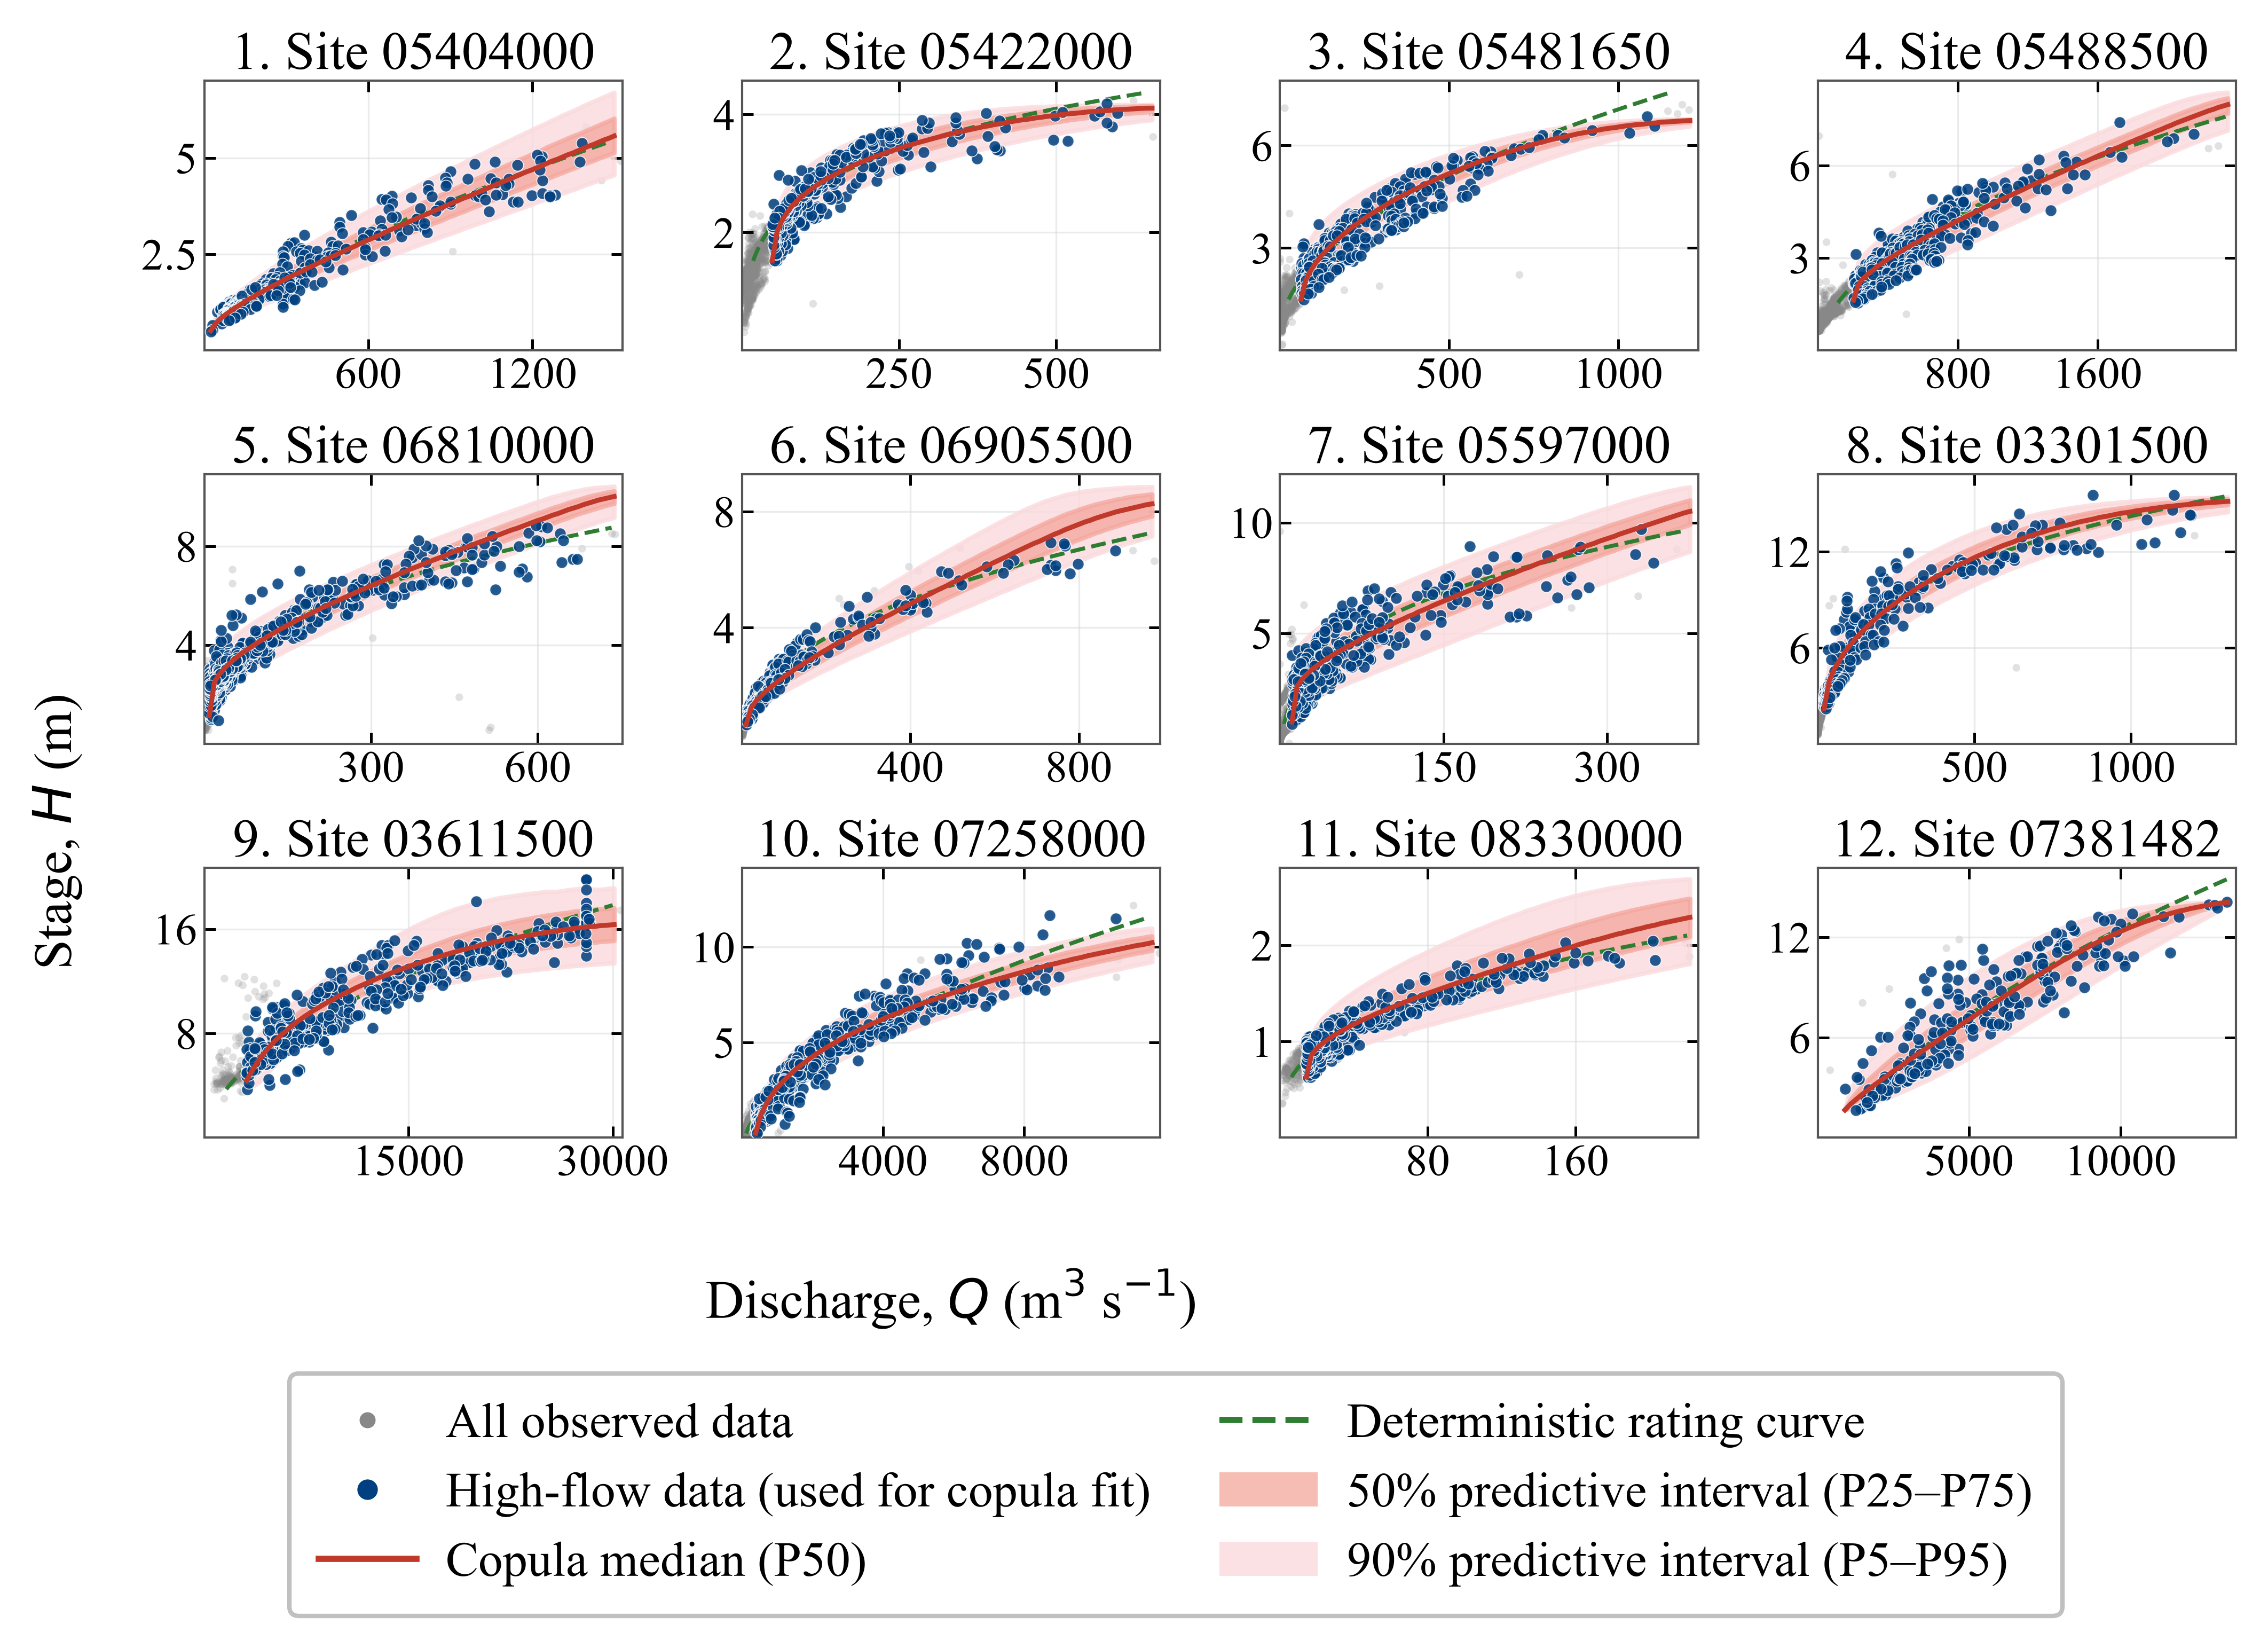
\includegraphics[width=\textwidth]{figs/fig-03.png}
    \caption{Probabilistic rating curves from the copula-based framework applied to representative IFMHA stations.}
    \label{fig:fig-03}
\end{figure}


\subsection{Case Studies}
The proposed framework is examined in detail at three USGS streamgages: the Little Sioux River at Correctionville (USGS 06606600), the Des Moines River near Saylorville (USGS 05481650), and the Brazos River at Waco (USGS 08096500). First, the predictive performance of the proposed copula-based framework is benchmarked against Gaussian Process Regression (GPR). Next, its practical implications for flood mapping are demonstrated by generating inundation maps for stage values corresponding to different conditional percentiles at a given discharge. This analysis shows how uncertainty in probabilistic stage estimates propagates into differences in predicted flood extent. Additional site characteristics, marginal-distribution fitting, and copula-family selection are provided in Appendix~\ref{app:case_studies}.

At the two Iowa sites (Figure~\ref{fig:fig-04}a, b), the median follows the deterministic rating curve closely across the full discharge range. At the Brazos River (Figure~\ref{fig:fig-04}c), the two diverge at high flow: the deterministic curve continues to rise, whereas the copula median follows the trend in the observed high-flow data. This divergence reflects the truncated Gaussian marginal fitted to stage at the Brazos River (Appendix~\ref{app:case_studies}). Its finite upper bound constrains the copula-based stage predictions, whereas the power-law rating curve remains unbounded.


\begin{figure}[htbp]
    \centering
    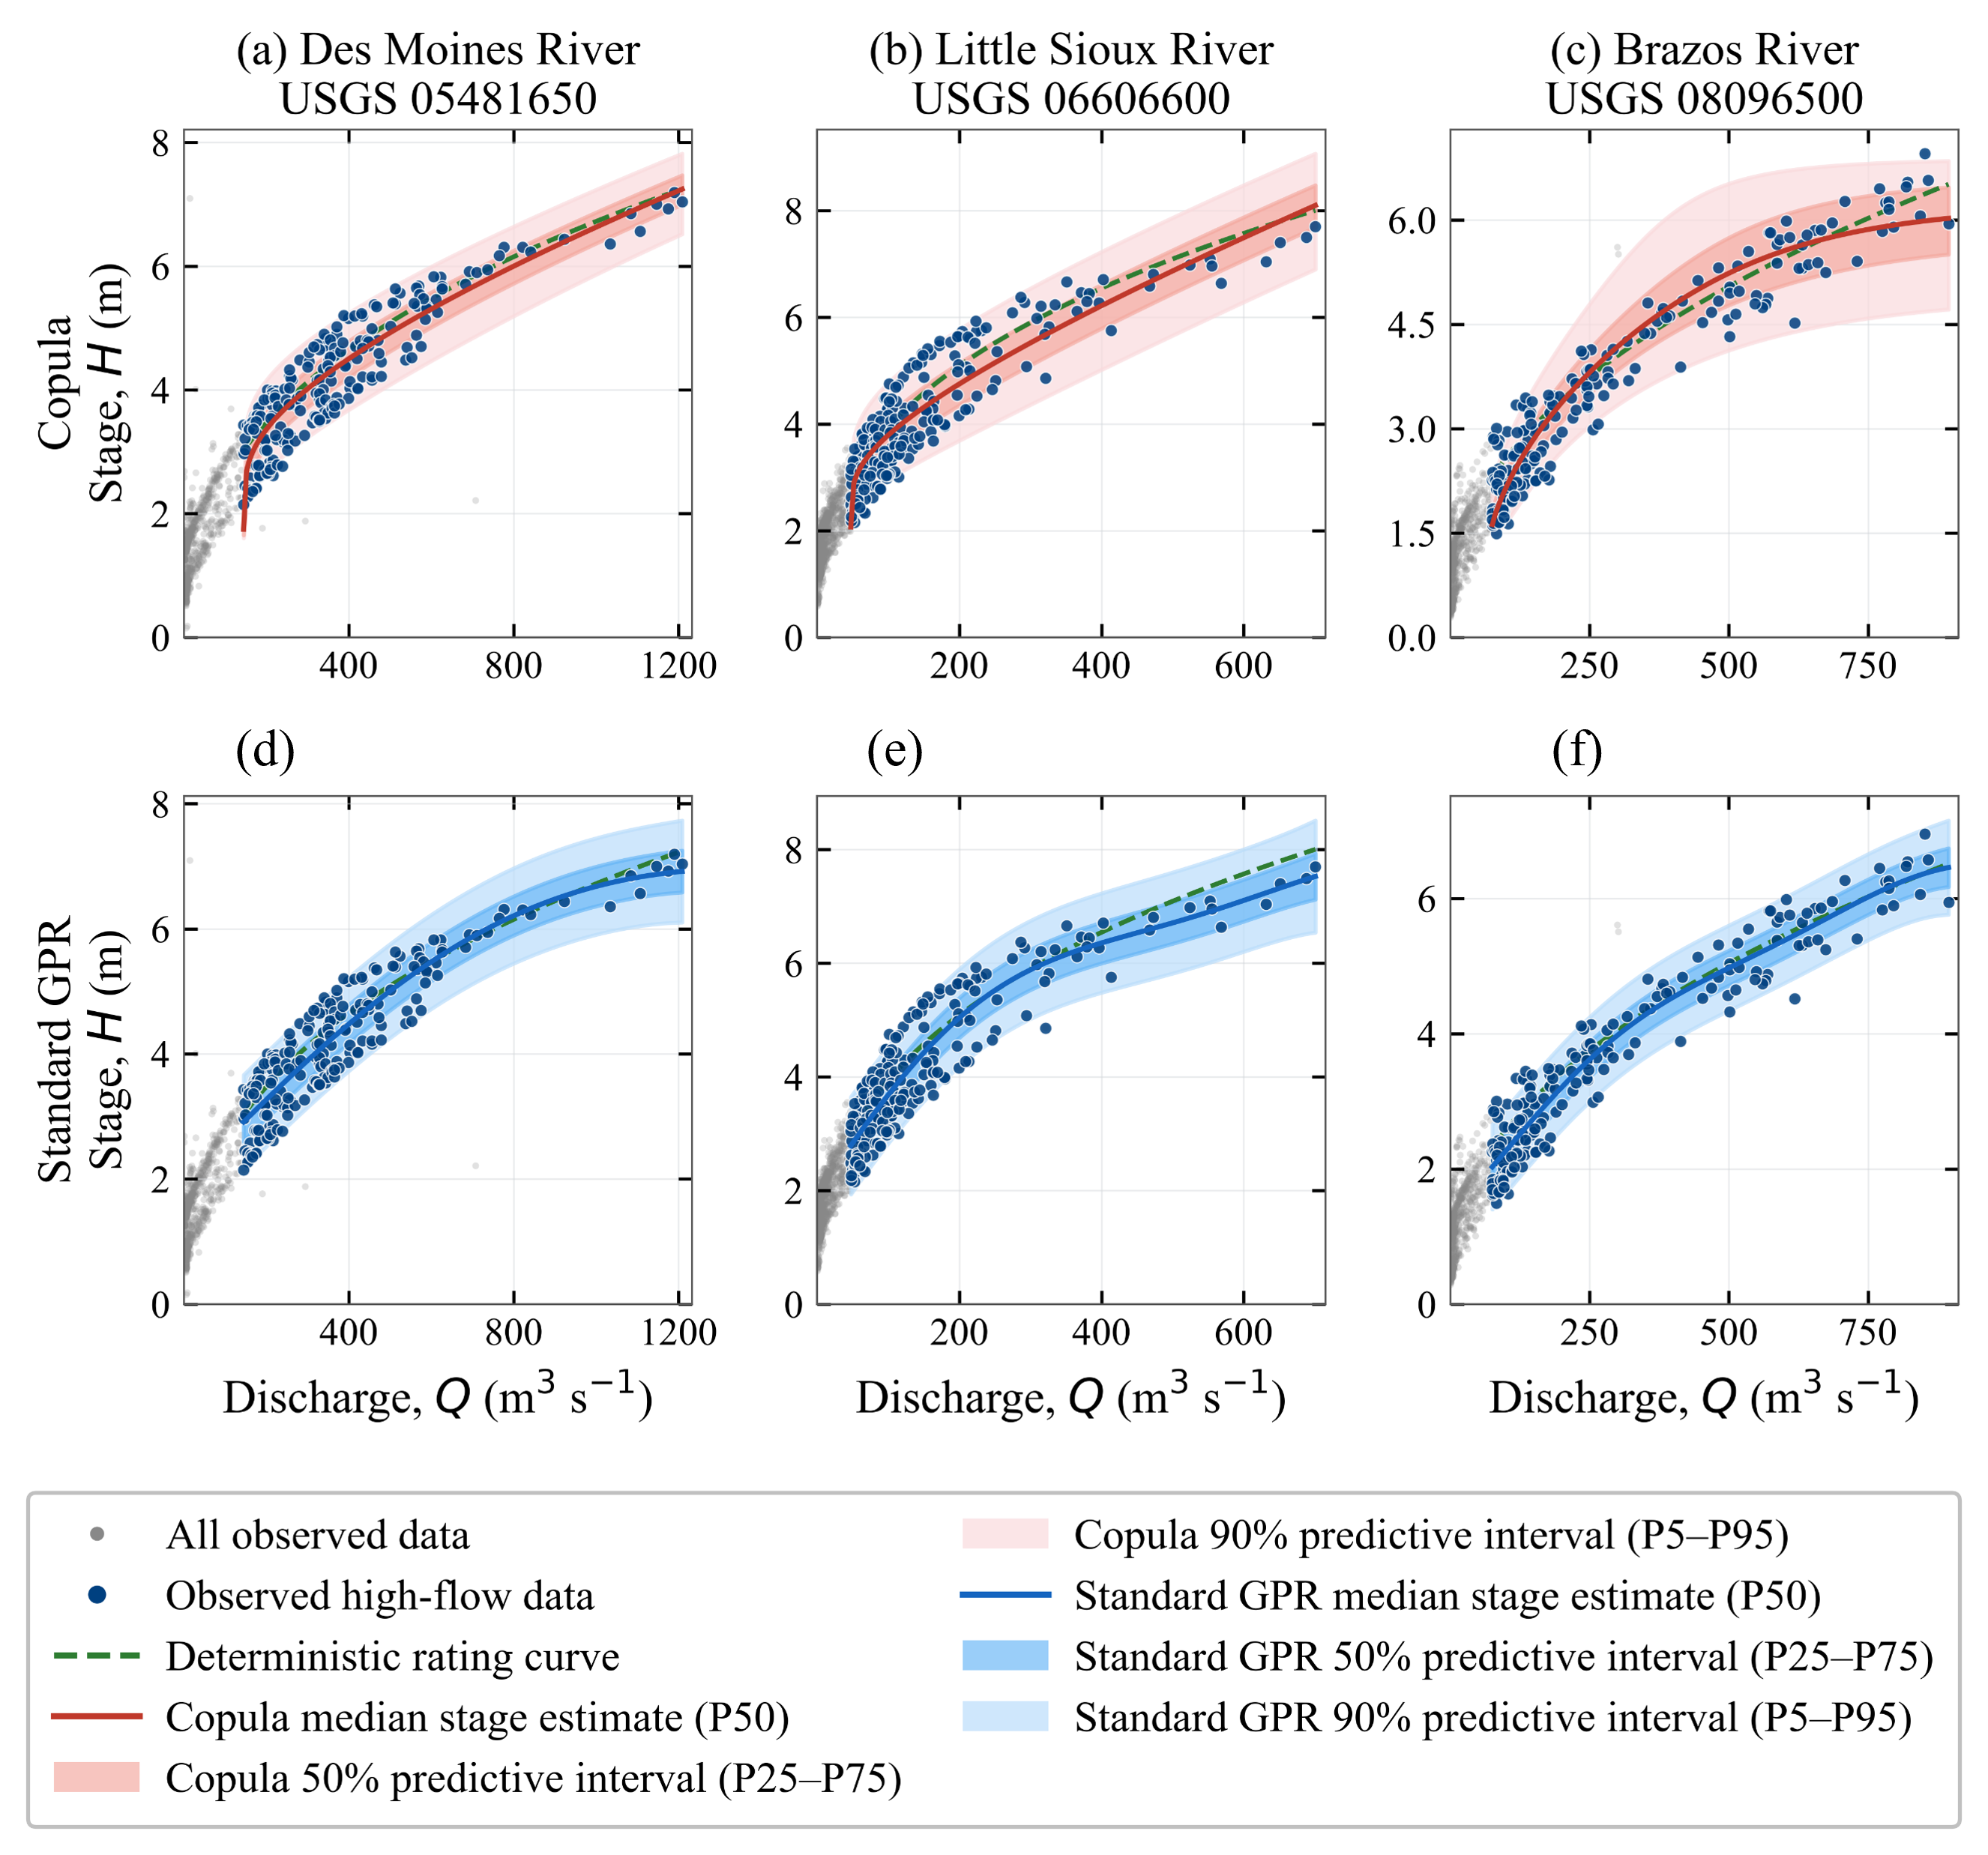
\includegraphics[width=\textwidth]{figs/fig-04.png}
    \caption{Probabilistic rating curves for the three case-study sites.}
    \label{fig:fig-04}
\end{figure}

The proposed framework is compared against GPR at three sites (05481650, 06606600, 08096500), using a standard formulation with homoscedastic noise. Both are fit to the same high-flow subset and the same configuration used for the copula. Both models are scored on 95\% interval coverage, average interval width, and the Continuous Ranked Probability Score (CRPS), which increases when predictions are miscalibrated or intervals are wider than necessary (see Table~\ref{tab:tab-02}).

\begin{table}[htbp]
    \centering
    \label{tab:tab-02}
    \caption{Predictive performance of the copula framework versus standard GPR at each site.}
    \begin{tabular}{lccc ccc}
        \toprule
        USGS Site & \multicolumn{3}{c}{Copula} & \multicolumn{3}{c}{Standard GPR} \\
        \cmidrule(lr){2-4} \cmidrule(lr){5-7}
        Number & Cov. (\%) & Width (m) & CRPS (m) & Cov. (\%) & Width (m) & CRPS (m) \\
        \midrule
            05481650 & 99.1 & 1.843 & 0.274 & 100.0 & 1.790 & 0.264 \\
            06606600 & 95.5 & 2.204 & 0.326 & 99.1  & 2.046 & 0.297 \\
            08096500 & 94.5 & 1.945 & 0.245 & 96.5  & 1.496 & 0.213 \\
        \bottomrule
    \end{tabular}

\end{table}

Both methods achieve coverage close to the nominal 95\% level, indicating that the copula's predictive intervals are well calibrated. On sharpness, the standard GPR attains the lowest CRPS and narrowest intervals at every site, with the copula performing comparably but not better. A Gaussian predictive distribution is symmetric by construction. A GPR's upper and lower half-intervals are therefore equal, and its conditional skewness is zero at every discharge, regardless of kernel or tuning. This is visible in Figure~\ref{fig:fig-04} ?? as the near-uniform bands in the bottom row. The copula is not subject to this constraint. At all three sites, its conditional distribution is right-skewed at low discharge (skewness up to $+1.1$) and left-skewed at high discharge (as low as $-0.7$). This is consistent with stage being bounded near the channel bed at low flow, and with the rating curve flattening at high flow. No GPR configuration reproduces this reversal.

The copula offers a second advantage that follows from how it is built. It models the joint distribution of discharge and stage. Both conditionals, $f(H \mid Q)$ and $f(Q \mid H)$, therefore follow from a single fit. The two serve opposite operational needs. At a gauging station, stage is monitored continuously and discharge is inferred from it. This is the task a conventional rating curve performs, and it calls for $f(Q \mid H)$. In flood inundation modeling the direction reverses.  Discharge comes from a hydrologic model or forecast, and the stage it would produce must be estimated. This calls for $f(H \mid Q)$. A regression, however, is fit in one direction only. Obtaining the reverse conditional would require a second, independently fit model, with no guarantee of consistency between the two. The copula supplies both from the same fit, and the two are consistent by construction. The copula framework matches a well-tuned GPR baseline on calibration and sharpness. It additionally offers an asymmetric, physically consistent predictive distribution and native bidirectional prediction, neither available from a regression-based baseline.

\subsubsection{Flood Inundation Mapping with Stochastic Rating Curve}
For each of the three case-study sites, the probabilistic rating curve is paired with the inundation extents at the 5th and 95th percentile stages as well as its corresponding synthetic rating curve (SRC) stage. It's worth noting that the 90\% prediction intervals used to produce the flood inundation maps come from a fitted copula distribution that has a appropriate spread metric and are not simply overestimating the range of uncertainty.

At the Little Sioux River (Figure~\ref{fig:fim_6606600}), a discharge of $Q = 400$~m$^3$~s$^{-1}$ corresponds to a stage range of $H_{P05} = 5.02~m$ to $H_{P95} = 7.23$~m (i.e., a spread of $2.21$~m). The lower bound stays confined to the channel corridor while the upper bound extends across the floodplain and covers the town of Correctionville. The HAND-FIM SRC ($H = 5.66$~m) falls between $H_{P05}$ and $H_{P25}$, near the 21st percentile.

% SITE 1: Little Sioux River
% ==============================================================
% \begin{figure}[H]
% \centering
% \begin{minipage}[t]{0.40\textwidth}
% \centering
% \includegraphics[width=\linewidth]{GUMBEL-6606600-SRC-Added-2.png}
% \end{minipage}\hfill
% \begin{minipage}[t]{0.57\textwidth}
% \centering
% \includegraphics[width=\linewidth]{6606600_FIM_final.png}
% \end{minipage}
% \caption{Little Sioux River at Correctionville (USGS 06606600) at
% $Q = 400$~m$^3$~s$^{-1}$. Left: probabilistic rating curve with the 5th
% ($H_{P05} = 5.02$~m) and 95th ($H_{P95} = 7.23$~m) percentile stage
% estimates and the HAND-FIM SRC ($H = 5.66$~m). Right: corresponding
% inundation extents for the lower bound, HAND-FIM SRC, and upper bound,
% overlaid.}
% \label{fig:fim_6606600}
% \end{figure}

At the Des Moines River (Figure~\ref{fig:fim_5481650}), a discharge of $Q = 600$~m$^3$~s$^{-1}$ yields $H_{P05} = 4.47$~m and $H_{P95} = 5.99$~m (i.e., a spread of 1.52~m). While small, this $1.52$~m difference produces a large change in inundated area: the flat Iowa terrain offers little topographic resistance, so the flood extent expands substantially between the lower and upper bounds. The SRC ($H = 5.17$~m) falls between $H_{P25}$ and $H_{P50}$, near the 38th percentile, closer to the median than at the Little Sioux River. Away from the main channel, both the SRC and upper-bound extents include isolated flooded patches over agricultural fields with no visible connection to the river. This is a known limitation of HAND: it assigns inundation by elevation threshold alone, without checking hydraulic connectivity. 

% ==============================================================
% % SITE 2: Des Moines River
% % ==============================================================
% \begin{figure}[H]
% \centering
% \begin{minipage}[t]{0.40\textwidth}
% \centering
% \includegraphics[width=\linewidth]{GUMBEL-5481650-SRC-Added-2.png}
% \end{minipage}\hfill
% \begin{minipage}[t]{0.57\textwidth}
% \centering
% \includegraphics[width=\linewidth]{5481650_FIM_final.png}
% \end{minipage}
% \caption{Des Moines River near Saylorville (USGS 05481650) at
% $Q = 600$~m$^3$~s$^{-1}$. Left: probabilistic rating curve with the 5th
% ($H_{P05} = 4.47$~m) and 95th ($H_{P95} = 5.99$~m) percentile stage
% estimates and the HAND-FIM SRC ($H = 5.17$~m). Right: corresponding
% inundation extents; panels as in Figure~\ref{fig:fim_6606600}.}
% \label{fig:fim_5481650}
% \end{figure}

At the Brazos River (Figure~\ref{fig:fim_8096500}), a discharge of $Q = 600$~m$^3$~s$^{-1}$ produces the widest stage range among the three sites. The 90\% predictive interval extends from $H_{P05} = 4.36$~m to $H_{P95} = 6.70$~m, corresponding to a spread of $2.34$~m. This stage uncertainty results in a substantial difference in the simulated flood extent between the lower- and upper-bound scenarios. Much of the additional area inundated under the upper-bound scenario extends into developed parts of Waco, indicating that uncertainty in stage estimates can materially affect estimates of urban flood exposure. The SRC ($H = 5.29$~m) falls between $H_{P25}$ and $H_{P50}$, near the 37th percentile.

% ==============================================================
% SITE 3: Brazos River
% ==============================================================
% \begin{figure}[H]
% \centering
% \begin{minipage}[t]{0.40\textwidth}
% \centering
% \includegraphics[width=\linewidth]{FRANK-8096500-SRC-added-2.png}
% \end{minipage}\hfill
% \begin{minipage}[t]{0.57\textwidth}
% \centering
% \includegraphics[width=\linewidth]{8096500_FIM_final.png}
% \end{minipage}
% \caption{Brazos River at Waco (USGS 08096500) at
% $Q = 600$~m$^3$~s$^{-1}$. Left: probabilistic rating curve with the 5th
% ($H_{P05} = 4.36$~m) and 95th ($H_{P95} = 6.70$~m) percentile stage
% estimates and the HAND-FIM SRC ($H = 5.29$~m). Right: corresponding
% inundation extents; panels as in Figure~\ref{fig:fim_6606600}.}
% \label{fig:fim_8096500}
% \end{figure}

Across all three sites, the SRC estimate fell below the copula median, corresponding to approximately the 21st to 38th conditional percentiles. Thus, for these case studies, the SRC cannot be characterized as conservative from a flood-hazard perspective. This finding does not imply that the SRC is unreliable; rather, a deterministic hydraulic estimate represents a single point within a range of plausible stage outcomes and does not, by itself, reveal its position within that range.
% The relative position of the SRC varied among the sites, lying closer to the lower bound at the unregulated Little Sioux River than at the dam-regulated Des Moines River or the urbanized Brazos River. Because only three sites were examined, this pattern should be treated as an observation rather than a general relationship.
The Brazos River case further demonstrates that stage uncertainty does not necessarily translate proportionally into inundation uncertainty: despite its wide stage range, the corresponding change in flood extent was relatively small because the local floodplain topography constrained lateral expansion. Taken together, these findings suggest that site-specific conditions influence both the position of the SRC within the probabilistic stage distribution and the extent to which stage uncertainty affects mapped inundation.

\section{Conclusion}
Accurately characterizing the stage--discharge relationship, and the uncertainties inherent to it, has long been a challenge in river hydraulics. This relationship is conventionally represented by a deterministic rating curve, yet it is inherently stochastic and cannot be fully captured by a single deterministic function. Here we introduced a copula-based probabilistic framework, drawing from multivariate probability theory, to model this relationship directly from field observations. The approach treats discharge and stage as jointly distributed random variables and estimates the conditional distribution of stage given discharge, $f(H \mid Q)$, without assuming a functional form or requiring site-specific hydraulic knowledge. 

A CONUS-scale analysis of 6,323 USGS gauges showed that this stochasticity is systematic rather than site-specific. Stage variability at fixed discharge is highest in the low-gradient alluvial region, and lowest in the steep, bedrock-controlled channels. This is the variability the framework is designed to represent. The framework was applied across sites spanning a range of drainage area, stream order, and hydrologic setting. It produced well-calibrated predictive intervals, with 95\% coverage between 94.1\% and 97.8\%. These results used a single uniform configuration rather than site-by-site calibration, which supports its transferability across such diverse settings.
% The framework matched a well-tuned Gaussian Process Regression on calibration while offering properties a regression cannot. It produces an asymmetric conditional distribution consistent with the physical bounds on stage, and yields consistent $f(H \mid Q)$ and $f(Q \mid H)$ from a single fit.
The framework's implications extend beyond the rating curve itself. Propagating the probabilistic stage estimates through the OWP HAND--FIM model showed that a single discharge yields a range of plausible inundation extents. This propagation is non-proportional and depends on local floodplain geometry.

Although the proposed framework requires no prior information about the hydraulic characteristics of a site, which is an advantage, it fits statistical models for both the marginals and the dependence structure. It therefore carries more degrees of freedom than a deterministic power law and needs a larger number of reliable observations to be well constrained.
% As a data-driven method, it also cannot yet be applied to ungauged reaches.
Future work could broaden the framework's reach. Regionalizing copula parameters using catchment and channel attributes such as drainage area, slope, and stream order would extend the approach to ungauged sites. The probabilistic estimates could also be integrated into NWM-based inundation mapping as uncertainty-aware complements to synthetic rating curves, or used to generate synthetic stage--discharge pairs where observations are sparse. The resulting distributions could further serve as an observation-error model for calibrating rainfall-runoff models directly in stage space, reducing the parameter bias introduced by ignoring rating-curve uncertainty~\citep{sikorska2017}. More broadly, acknowledging the stochastic nature of the stage-discharge relationship supports more realistic and risk-aware decisions in streamflow forecasting, infrastructure design, sediment and water-quality modeling, and water-resources planning.

\newpage
\bibliographystyle{unsrt}
\bibliography{ref.bib}

% \newpage \appendix

\end{document}